\section{\textit{session-rec}} A biblioteca \textit{session-rec} foi
desenvolvida para facilitar experimentos comparando recomendadores
\textit{session-based} em Python. A biblioteca contém as implementações dos
modelos previamente citados no presente trabalho. Um novo modelo pode ser
implementado seguindo o polimofismo das demais implementações.

Cada experimento é declarado em um arquivo .yml, contendo as informações dos
dados a serem utilizados, dos modelos a serem avaliados e de seus hiperparâmetros.

A biblioteca contém um script de pré--processamento, responsável por separar os
dados em conjuntos de treinamento, validação e teste, filtrando os dados de
acordo com o suporte mínimo dos itens e o número mínimo de usuários por sessão,
à escolha do usuário. Em geral, os conjuntos de testes nos comparativos
publicados utilizando a ferramenta é limitado a itens nos dias mais recentes, da
ordem de 1 a 7 dias.

A divisão dos dados pode ser feita de duas formas: \textit{single split} e
\textit{window}. A primeira forma divide o conjunto de dados em um único
conjunto de teste e treinamento. A segunda forma divide a base de dados em
múltiplos conjuntos de acordo com uma janela de tempo especificada. Dessa forma, os
últimos dias de cada conjunto são reservados para teste, enquanto que os dias
anteriores da mesma janela são utilizados para o treinamento.

 Entre os métodos de avaliação disponíveis na biblioteca, há dois mais
 utilizados em publicações com os comparativos: no primeiro, avalia-se a
 capacidade de prever o próximo item imediato da sessão. No segundo, avalia-se a
 capacidade de prever todos os itens subsequentes da sessão.

 O presente trabalho utiliza também uma terceira forma de avaliação, em que
 avalia-se apenas o último item da sessão.

\section{Análise preliminar dos dados}

Os dados utilizados neste trabalho consistem nas sessões de gravação no
Indaband, no período compreendido entre 01 de janeiro de 2023 até 19 de dezembro
de 2023.

% Metric                         Value
% ---------------------------  -------
% Sessions created               93314
% Sessions published             18845
% Users who added tracks         11968
% Users with published tracks     3630
% Tracks added                  457224
% Fork tracks                   349060
% Tracks published              134004

\begin{table}[H]
  \centering
  \begin{tabular}{|l|l|}
    \hline
    \textbf{Período} & 01/01/2023 a 19/12/2023 \\ \hline
    Sessões criadas & 93.314 \\ \hline
    Sessões publicadas & 18.845 \\ \hline
    Usuários que adicionaram faixas & 11.968 \\ \hline
    Usuários com faixas publicadas & 3.630 \\ \hline
    Faixas adicionadas & 457.224 \\ \hline
    Faixas \textit{forkadas} & 349.060 \\ \hline
    Faixas publicadas & 134.004 \\ \hline
  \end{tabular}
  \caption{Quantidade de sessões, faixas e usuários no período de 01/01/2023 a 19/12/2023.}
  \label{tab_sessoes}
\end{table}

Verifica-se na tabela \ref{tab_sessoes} uma grande quantidade de faixas criadas,
\textit{forkadas} e publicadas na plataforma. Essas faixas são criadas por um
número pequeno de usuários. Por sua vez, na tabela \ref{tab_convites}, a
quantidade de convites enviados e aceitos é ainda menor em relação ao número de
usuários ativos no período.

\begin{table}[htbp]
  \centering
  \begin{tabular}{|l|l|}
    \hline
    \textbf{Período} & 01/01/2023 a 19/12/2023 \\ \hline
    Sessões criadas & 93.315 \\ \hline
    Sessões com convites & 3.984 \\ \hline
    Sessões com participantes & 1.388 \\ \hline
    Convites & 4.619 \\ \hline
    Convites aceitos & 2.799 \\ \hline
    Usuários que convidaram & 592 \\ \hline
    Usuários convidados & 934 \\ \hline
    Usuários que aceitaram convites & 652 \\ \hline
  \end{tabular}
  \caption{Informações sobre convites no período de 01/01/2023 a 19/12/2023.}
  \label{tab_convites}
\end{table}

Em razão desses dois aspectos, o sistema de recomendação \textit{session-based}
proposto prevê qual o próximo usuário cuja faixa será incluída na sessão, dados
os demais usuários com faixas inclusas e do histórico de sessões dos usuários
envolvidos. Por mais que essa abordagem não utilize os convites, ela é capaz de
recomendar usuários que ainda não tenham contribuído para a sessão e que
potencialmente possam contribuir.

Dessa forma, os itens das sessões serão os próprios usuários, e não as faixas,
evitando que o sistema recomende um usuário que já tenha uma faixa incluída na
sessão. Além disso, seguindo a abordagem \textit{session-aware}, o criador de
cada sessão será considerado como o usuário ativo. Isso permite que o sistema
modele as preferências individuais de usuários ao criarem sessões.

Em razão da modelagem apresentada, os padrões mais esperados para os modelos são:

\begin{itemize}
  \item Usuários que co-participem de sessões e tendem a repetir as
  colaborações serem previstos corretamente como próximo usuário e recomendados;
  \item Sessões com muitos \textit{forks} sejam mais fáceis de prever o próximo
  usuário e os usuários restantes, uma vez que a base de dados contém diferentes
  variações dessas sessões e de seus \textit{forks};
  \item Na abordagem \textit{session-based}, a predição do último usuário da
sessão erre mais do que a predição do próximo usuário e do que a dos
usuários restantes, por tratar-se de um item inédito tanto naquela sessão quanto
nas sessões precedentes no caso de um \textit{fork};
  \item Que na abordagem \textit{session-based}, usuários que se isolam e que
 praticam a partir de \textit{forks} de outros usuários, sem necessariamente
 publicar suas versões, sejam previstos incorretamente como o próximo usuário
 para sessões de outros usuários e recomendado -- o que não necessariamente
 seria algo negativo, sob o ponto de vista de integrá-lo à comunidade -- e que esse
 mesmo comportamento não seja observado na abordagem \textit{session-aware}, uma vez que 
 há a informação do dono da sessão;
  \item Na abordagem \textit{session-aware}, que os principais colaboradores de
  determinado dono da sessão sejam recomendados, por mais que ambos não constem como
  itens na sessão.
\end{itemize}

 \section{Bases de comparação}
 A seguir, são apresentadas as bases de dados utilizadas na bibliografia de
  SBRS. O domínio de cada uma dessas bases é de comércio eletrônico, música e
  notícias. Os valores das tabelas \ref{tab:datasets} e
  \ref{tab:datasets_comparison} foram retirados de \citet{ludewig_2018}.

  Observa-se que a base de dados do Indaband é a menor dentre as bases
  de dados disponíveis, considerando quantidade de interações, sessões e itens
  distintos. Isso se deve a dois motivos: primeiramente, a modelagem do problema
  como recomendação do próximo usuário filtra uma grande quantidade de
  interações, uma vez que o mesmo usuário grava várias faixas em uma mesma
  sessão. Em razão disso, a quantidade de itens únicos por sessão é mais enxuta.
  Além disso, a aplicação é mais recente que as demais, em fase de crescimento e
  aquisição de usuários.

  \begin{table}[htbp]
    \centering
    \begin{tabular}{lcccccc}
        \toprule
        \textbf{Dataset} & \textbf{RSC15-S} & \textbf{RSC15} & \textbf{TMALL} & \textbf{RETAILR} & \textbf{ZALANDO} \\
        \midrule
        Interações & 31.71M & 5.43M & 13.42M & 212.182 & 4.54M \\
        Sessões & 7.98M & 1.38M & 1.77M & 59.962 & 365.126 \\
        Itens & 37.483 & 28.582 & 425.348 & 31.968 & 189.328 \\
        Dias & 182 & 31 & 91 & 27 & 91 \\
        \hline
        Interações por sessão & 3,97 & 3,95 & 7,56 & 3,54 & 12,43 \\ 
        Itens únicos por sessão & 3,17 & 3,17 & 5,56 & 2,56 & 8,39 \\ 
        Interações por dia & 174,222 & 175,063 & 149,096 & 7,858 & 50,410 \\
        Sessões por dia & 43,854 & 44,358 & 19,719 & 2,220 & 4056 \\ 
        \bottomrule
    \end{tabular}
    \caption{Distribuição dos dados nos conjuntos de comércio eletrônico. O
    conjunto RSC15-S é a versão \textit{single-split} do conjunto RSC15. Os demais
    conjuntos são a média de 5 \textit{splits}. }
    \label{tab:datasets}
  \end{table}
  
  \begin{table}
    \centering
    \begin{tabular}{lcccccc}
        \toprule
        \textbf{Dataset} & \textbf{8TRACKS} & \textbf{30MUSIC} & \textbf{AOTM} & \textbf{NOW PLAYING} & \textbf{CLEF} \\
        \midrule
        Interações & 1.50M & 638.933 & 306.830 & 271.177 & 5.54M \\
        Sessões & 132.453 & 37.333 & 21.888 & 27.005 & 1.64M \\
        Itens & 376.422 & 210.633 & 91.166 & 75.169 & 742 \\
        Dias & 95 & 95 & 95 & 95 & 6 \\
        \hline
        Interações por sessão & 11,32 & 17,11 & 14,02 & 10,04 & 3,37 \\
        Itens únicos por sessão & 11,31 & 14,47 & 14,01 & 9,38 & 3,17 \\
        Interações por dia & 16.663 & 7.099 & 3.409 & 3.013 & 923.414 \\
        Sessões por dia & 1.472 & 415 & 243 & 300 & 274.074 \\
        \bottomrule
    \end{tabular}
    \caption{Distribuição dos dados nos conjuntos de música e notícias, média dos cinco \textit{splits}.}
    \label{tab:datasets_comparison}
  \end{table}
  
  \begin{table}
    \centering
    \begin{tabular}{lcc}
        \toprule
        \textbf{Dataset} & \textbf{INDA \textit{single}} & \textbf{INDA \textit{windowed}}\\
        \midrule
        Interações & 102.066 & 17.184  \\
        Sessões & 29.755 & 5.068  \\
        Itens & 1702 & 615  \\
        Dias & 351 & 67  \\
        \hline
        Interações por sessão & 3,43 & 3,23 \\
        Itens únicos por sessão & 3,43 & 3,23 \\
        Interações por dia & 290 & 50 \\
        Sessões por dia & 85 & 18 \\
        \bottomrule
    \end{tabular}
    \caption{Análise dos conjuntos de dados do Indaband.}
    \label{tab:datasets_including_inda}
  \end{table}
  
  \section{Experimentos} 

% \begin{table}[htbp]
%   \centering
%   \begin{tabular}{|l|l|l|l|}
%     \hline
%       & Eventos & Sessões & Itens \\ \hline
%      \textit{Dataset} completo & 154.121 & 77.055 & 20.840 \\ \hline
%       \textit{Dataset} filtrado & 105.955 & 31.103 & 2.579 \\ \hline
%       Conjunto completo de treinamento & 99.714 & 29.328 & 2.452 \\ \hline
%       conjunto de teste & 5.516 & 1.530 & 477 \\ \hline
%       Conjunto de treinamento & 93.679 & 27.605 & 2.320 \\ \hline
%       Conjunto de validação & 5.291 & 1.467 & 475 \\ \hline
%       Conjunto de otimização & 304 & 100 & 111 \\ \hline
%   \end{tabular}
%   \caption{Informações sobre o \textit{dataset} utilizado na abordagem \textit{single}.}
%   \label{tab_dataset}
% \end{table}

\subsection{Abordagem \textit{single-split}, \textit{session-based}, \textit{next-item}}

\citet{HidasiKBT15} utiliza a abordagem \textit{single-split} para comparar a
avaliação dos modelos, de forma que o conjunto de treinamento é composto pelos
últimos seis meses, enquanto que o conjunto de teste é composto pelo último dia
do conjunto completo \cite{ludewig_2018}. Essa é a abordagem mais próxima de um
modelo em produção.

O \textit{dataset} é dividido segundo a abordagem \textit{single split}, em um
único conjunto de treinamento e teste, tal como na tabela
\ref{tab:split_data}. Nesses experimentos, os modelos de base de comparação
desconsideram o usuário dono da sessão. Dessa forma, não há modelos
\textit{session-aware}.

Apenas sessões com um mínimo de dois usuários estão presentes, como ilustrado na
figura \ref{fig:next-item-single}. Similarmente, o suporte mínimo dos itens é
igual a 2. Dessa forma, há apenas usuários que constam em pelo menos duas
sessões publicadas. Essa abordagem é distinta da maioria dos comparativos, que
utilizam suporte mínimo igual a 3. Essa decisão foi tomada pela menor quantidade
de dados disponíveis, em comparação com as demais bases de dados. Essa distanção
é necessária ser destacada, em razão do eventual uso desses dados
para comparativos com outras bases. Uma vez que o foco do presente trabalho é a
avaliação dentro do contexto da aplicação, essa foi a decisão mais adequada para
manter a maior quantidade de dados possível.

Na abordagem apresentada, apenas a primeira interação de cada usuário na
sessão consta na base, de forma que nenhum usuário apareça mais de uma vez na
mesma sessão. Dessa forma, a tarefa do modelo é prever qual será o próximo usuário
inédito a contribuir na sessão.


  \begin{table}[htbp]
    \centering
    \begin{tabular}{|l|l|l|l|l|l|l|}
      \hline
      Conjunto & Eventos & Sessões & Itens & $\Delta$ & $\sigma$ & Janela de tempo \\ \hline 
         Treinamento & 90.801 & 26.649 & 1.702 & 3,3 & 2,0 & 01/01/2023 a 03/12/2023 \\ \hline
        Teste & 11.265 & 3.106 & 589 & 3,6 & 2,0 & 02/08/2023 a 18/12/2023 \\ \hline
    \end{tabular}
    \caption{Informações sobre o \textit{dataset} utilizado na abordagem
    \textit{single}. $\Delta$ e $\sigma$ são a média e o desvio padrão da quantidade de
    usuários por sessão.}
    \label{tab:split_data}
  \end{table}

  \begin{figure}[ht]
    \centering
    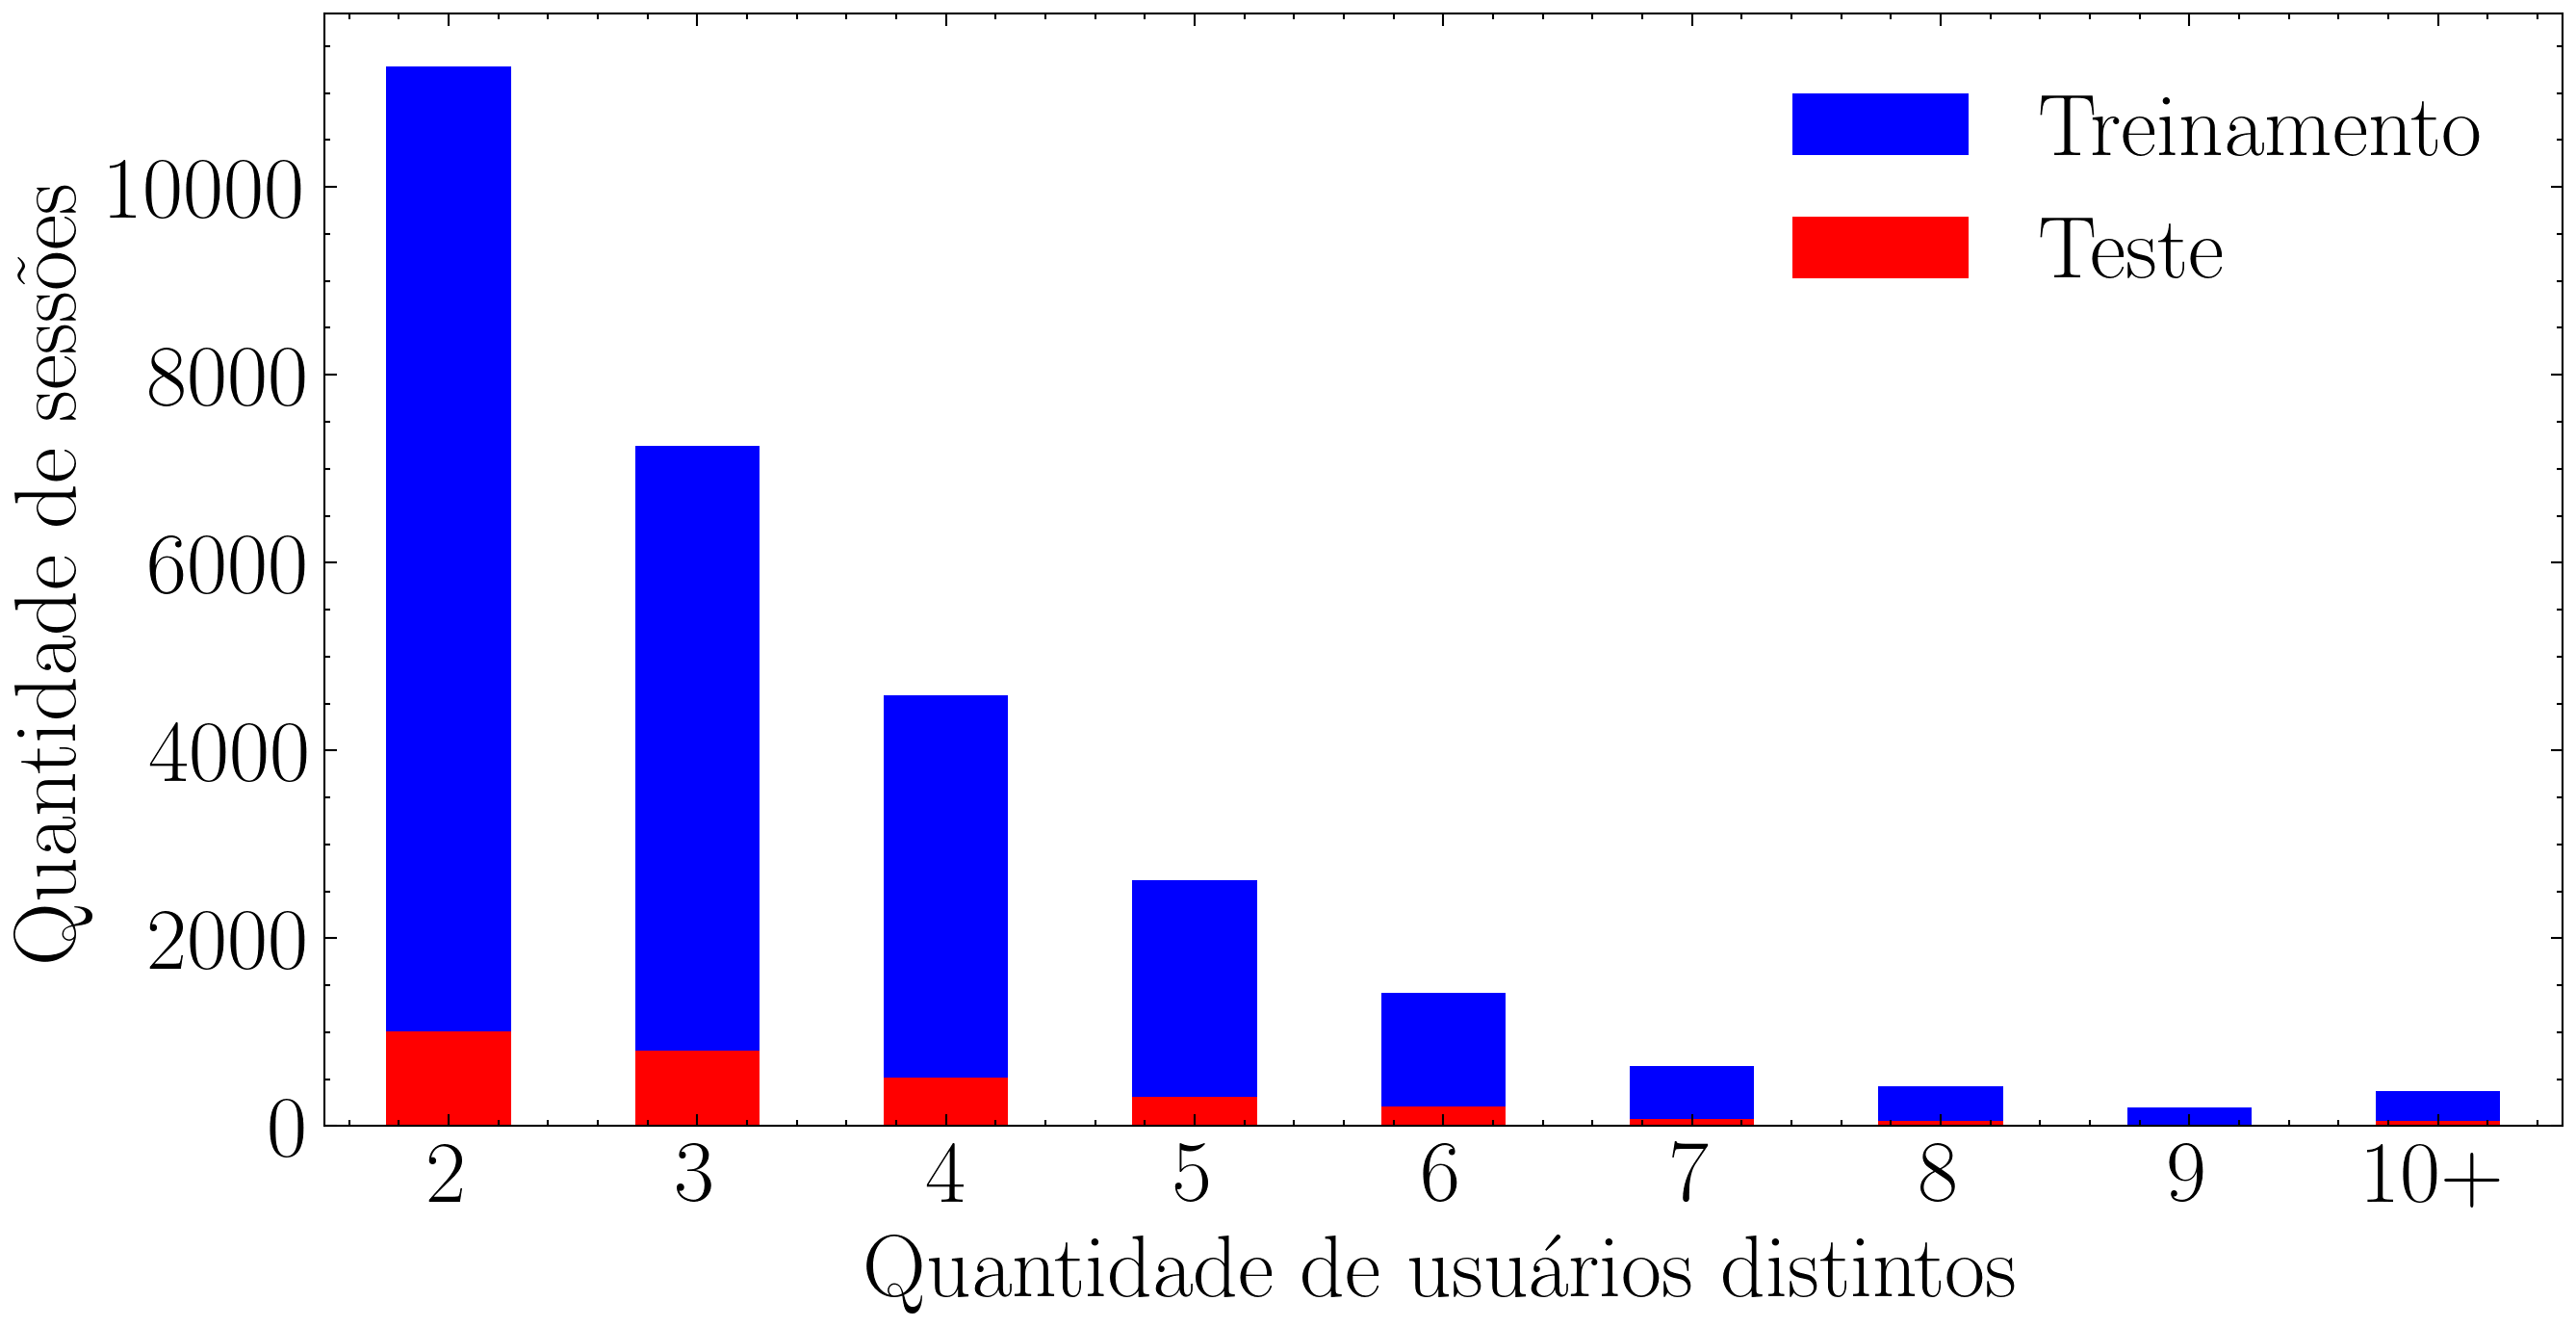
\includegraphics[width=1\textwidth]{chapters/chap04/images/histograma.png}
    \caption{Distribuição da quantidade de usuários por sessão na abordagem
    \textit{single}. A distribuição de treinamento está empilhada acima da
    distribuição de teste.}
    \label{fig:next-item-single}
  \end{figure}
 

  \subsubsection{Modelos não-personalizados}

  Pop é o modelo de popularidade, com pontuações proporcionais ao suporte dos
  itens, limitado aos 100 itens mais populares. Random é o modelo aleatório,
  retornando uma pontuação aleatória para cada item. SPop é o modelo de
  popularidade de sessão, em que as pontuações são proporcionais à maior
  frequência dos itens em cada sessão, também limitado aos 100 itens mais
  populares. Finalmente, RPop é o modelo de popularidade para sessões recentes,
  em que apenas itens do último dia são considerados por padrão. Foi utilizada a
  avaliação sobre o próximo item da sessão.
\begin{table}[htbp]
  \centering
  \begin{tabular}
    {|l|l|l|l|l|l|l|l|}
    \hline
    Modelo & HR@5 & HR@10 & MRR@5 & MRR@10 & NDCG@10 & Cov@10 & Pop@10 \\ \hline
    Pop & 0,132 & 0,268 & 0,092 & 0,110 & 0,155 & 0,006 & 0,531 \\ \hline
    Random & 0,003 & 0,006 & 0,001 & 0,002 & 0,003 & \textbf{1,000} & \textbf{0,013} \\ \hline
    RPop & \textbf{0,204} & \textbf{0,294} & \textbf{0,125} & \textbf{0,137} & \textbf{0,204} & 0,010 & 0,321 \\ \hline
    SPop & 0,109 & 0,221 & 0,045 & 0,058 & 0,114 & 0,301 & 0,473 \\ \hline
  \end{tabular}
  \caption{Resultados obtidos com os modelos de base de comparação não-personalizados, avaliando a predição do próximo item da sessão.}
\end{table}

De forma esperada, o modelo Random maximiza a cobertura, minimizando o índice de
popularidade. O modelo de popularidade para sessões recentes (RPop) apresenta
resultados superiores aos demais modelos de popularidade.


\subsubsection{Modelos por mineração de padrões e vizinhança}

\begin{table}[htbp]
  \centering
  \begin{tabular}{|l|l|l|l|l|l|l|l|}
    \hline
    Modelo & HR@5 & HR@10 & MRR@5 & MRR@10 & Cov@10 & Pop@10 & $\Delta t_{treino} [s]$ \\
    \hline
    ct & \textbf{0,541} & \textbf{0,631} & \textbf{0,392} & \textbf{0,404} & 0,518 & 0,358 & 8,3 \\
    \hline        
    $\text{SR}_{2}$ & 0,468 & 0,593 & 0,292 & \textbf{0,310} & 0,507 & 0,260 & 0,1 \\
    \hline
    Markov  & 0,465 & 0,583 & 0,292 & 0,308 & 0,488 & 0,247 & 0,1 \\
    \hline
    $\text{SR}_{1}$ & 0,461 & 0,583 & 0,291 & 0,308 & 0,492 & 0,272 & 0,1 \\
    \hline
    $\text{skNN}_{2}$ & 0,444 & 0,604 & 0,157 & 0,179 & 0,603 & 0,217 & 0,1 \\
    \hline
    $vstan_{1}$ & 0,419 & 0,573 & 0,161 & 0,182 & 0,553 & 0,230 & 0,1 \\
    \hline
    $vstan_{2}$ & 0,412 & 0,582 & 0,148 & 0,171 & 0,571 & 0,236 & 0,1 \\
    \hline
    $\text{skNN}_{1}$ & 0,406 & 0,564 & 0,151 & 0,172 & \textbf{0,636} & \textbf{0,187} & 0,1 \\
    \hline
    AR & 0,403 & 0,531 & 0,238 & 0,255 & 0,488 & 0,284 & 0.1 \\
    \hline
    $stan_{1}$ & 0,403 & 0,570 & 0,147 & 0,170 & 0,516 & 0,271 & 0.1 \\
    \hline
    $stan_{2}$ & 0,366 & 0,551 & 0,126 & 0,151 & 0,562 & 0,196 & 0.1 \\
    \hline
$\text{vsKNN}_{1}$ & 0,365 & 0,527 & 0,136 & 0,158 & 0,312 & 0,222 & 0.1 \\
    \hline
%     Metrics;HitRate@5: ;HitRate@10: ;MRR@5: ;MRR@10: ;Coverage@10: ;Popularity@10: ;
% ct;0.5418556195612207;0.6307145483515136;0.3915941496098388;0.4036660752465399;0.517626321974148;0.3575665829610209;
      \end{tabular}
  \caption{Resultado para os modelos de base de comparação, avaliando o próximo item da sessão.
  Os hiperparâmetros utilizados para cada modelo estão descritos no apêndice.}
  %  $\text{SR}_{1}$
  % e $\text{SR}_{2}$ são os modelos de regras de sequência com 6 e 11 passos, com peso inverso e quadrático.
  % $\text{skNN}_{1}$ e $\text{skNN}_{2}$ são os modelos de kNN com 50 e 100 vizinhos, ambos com função de similaridade cosseno.
  % $\text{vsKNN}_{1}$ e $\text{vsKNN}_{2}$ são os modelos de kNN com 1500 e 50 vizinhos, com amostragem de 10.000 e 2.500, respectivamente, ambos com função de similaridade cosseno.
  % vstan-k=1000-sample_size=5000-similarity=cosine-lambda_spw=10-lambda_snh=40-lambda_inh=5-lambda_ipw=1e-05-lambda_idf=False
  % vstan-k=2000-sample_size=1000-similarity=vec-lambda_spw=10-lambda_snh=100-lambda_inh=0.625-lambda_ipw=0.125-lambda_idf=False
  % $stan_{1}$ e $stan_{2}$ são os modelos de kNN com 1000 e 2000 vizinhos, com
  % amostragem de 5000 e 1000, respectivamente, com função de similaridade
  % cosseno e vetorial,   
  \label{tab_baseline}  
\end{table}

Em seguida, é realizada a avaliação para predição do próximo item em modelos de
mineração de padrões: regras de associação, cadeias de Markov, regras de
sequência. Também é realizada para métodos de vizinhança: kNN, vskNN, stan e
vstan. Os modelos SR, skNN e vsKNN são otimizados com seus respectivos
hiperparâmetros, obtidos a partir de uma otimização do MRR@10, cujas
métricas constam na tabela \ref{tab_baseline}.

Os modelos de regras de sequência e baseado em cadeias de Markov apresentam
resultados superiores, considerando as métricas HR@5, HR@10 e MRR@5 e MRR@10.
Apesar dos modelos de vizinhança não apresentarem resultados inferiores de HitRate,
o MRR decai consideravelmente.

\subsubsection{métodos baseados em fatoração}
Em seguida, são avaliados os modelos baseados em fatoração: FPMC, FISM, Fossil,
BPRMF e smf. Os resultados estão apresentados na tabela \ref{tab_fatoracao}.

\begin{table}[htbp]
  \centering
  \begin{tabular}{|l|l|l|l|l|l|l|l|}
    \hline
    Modelo & HR@5 & HR@10 & MRR@5 & MRR@10 & Cov@10 & Pop@10 & $\Delta t_{treino} [s]$ \\
    \hline
    $\text{smf}_1$ & \textbf{0,521} & \textbf{0,637} & \textbf{0,339} & \textbf{0,354} & 0,613 & 0,228 & 1146,6 \\
    \hline
    $\text{smf}_2$ & 0,506 & 0,616 & 0,332 & 0,346 & 0,321 & 0,256 & 987,4 \\
    \hline
    FPMC & 0,289 & 0,421 & 0,122 & 0,140 & 0,840 & \textbf{0,226} & 921,7 \\
    \hline
    FISM & 0,280 & 0,414 & 0,126 & 0,144 & 0,824 & 0,264 & 918,7 \\
    \hline
    BPRMF & 0,253 & 0,397 & 0,107 & 0,125 & 0,834 & 0,233 & 918,3 \\
    \hline
    Fossil & 0,243 & 0,399 & 0,100 & 0,121 & \textbf{0,848} & 0,253 & 917,7 \\
    \hline
        \end{tabular}
  \caption{Resultado para os modelos baseados em fatoração, avaliando o próximo item da sessão.}
  \label{tab_fatoracao}
\end{table}

Os modelos smf apresentam resultados superiores aos demais modelos, tanto no
HitRate quanto no MRR. Vale observar que o tempo de treinamento desses modelos é
muito mais demorado que os de mineração de padrões e vizinhança.

\subsubsection{Modelos baseados em redes neurais}
Em seguida, são avaliados os modelos baseados em redes neurais: GRU4Rec, NARM,
NextItNet, STAMP, GNN e Caser. Os resultados constam na tabela \ref{tab_nn_next_item}.

% Metrics;HitRate@5: ;HitRate@10: ;MRR@5: ;MRR@10: ;Coverage@10: ;Popularity@10: ;Saver@10: ;Training time:;Testing time seconds:;Testing time cpu:;
% narm-best-epochs=20-lr=0.006-hidden_units=100-factors=50;0.2931;0.39379;0.1730;0.18642;0.7179788;0.219598;1;6633.72;0.00666;0.00666;
% narm-second-epochs=20-lr=0.01-hidden_units=50-factors=50;0.27319;0.37712;0.1650;0.1786;0.69858989;0.213359;1;2598.844;0.00562;0.00562;

\begin{table}[htbp]
  \centering
  \begin{tabular}{|l|l|l|l|l|l|l|l|}
  \hline
  Modelo & HR@5 & HR@10 & MRR@5 & MRR@10 & Cov@10 & Pop@10 & $\Delta t_{treino} [s]$ \\
  \hline
  $\text{GNN}_1$ & \textbf{0,594} & \textbf{0,666} & \textbf{0,439} & \textbf{0,450} & 0,749 & 0,221 & 483,7 \\
  \hline
  $\text{GNN}_2$ & 0,588 & \textbf{0,666} & 0,425 & 0,435 & 0,713 & 0,220 & 464,6 \\
  \hline
  $\text{STAMP}_1$ & 0,543 & 0,639 & 0,385 & 0,398 & 0,672 & 0,244 & 106,6 \\
  \hline
  $\text{STAMP}_2$ & 0,539 & 0,638 & 0,384 & 0,397 & 0,635 & 0,243 & 106,6 \\
  \hline  
  $\text{NextItNet}_1$ & 0,426 & 0,526 & 0,277 & 0,290 & 0,336 & 0,278 & 1205,7 \\
  \hline
  $\text{NextItNet}_2$ & 0,410 & 0,518 & 0,278 & 0,293 & 0,312 & 0,287 & 966,4 \\
  \hline
  $\text{NARM}_1$ & 0,293 & 0,394 & 0,173 & 0,186 & \textbf{0,718} & 0,220 & 6633,7 \\
  \hline
  $\text{NARM}_2$ &  0,273 & 0,377 & 0,165 & 0,179 & 0,699 & \textbf{0,213} & 2598,8 \\
  \hline
  $\text{GRU4Rec}$ & 0,062 & 0,071 & 0,044 & 0,045 & 0,643 & 0,005 & 542,3 \\
  \hline
  $\text{CSRM}_1$ & 0.229 & 0.315 & 0.134 & 0.146 & 0.623 & 0.148 &  128,5 \\
  \hline
  $\text{CSRM}_2$ & 0.237 & 0.328 & 0.143 & 0.155 & 0.640 & 0.158 & 127,4 \\
  \hline
\end{tabular}
  \caption{Resultado para os modelos baseados em redes neurais, avaliando o próximo item da sessão.}
  \label{tab_nn_next_item}
\end{table}

Os modelos GNN e STAMP apresentam resultados superiores aos demais modelos de
redes neurais. São os modelos com melhor resultado entre todos da abordagem
\textit{single}.

% plot two plots at each size horizontally

% \begin{figure}[htbp]
%   \begin{subfigure}{0.5\textwidth}
%     \centering
%     \includegraphics[width=1\linewidth]{chapters/chap04/images/plotHitRate_n.png}
%     \caption{Plot 1}
%   \end{subfigure}%
%   \begin{subfigure}{0.5\textwidth}
%     \centering
%     \includegraphics[width=1\linewidth]{chapters/chap04/images/plotMRR_n.png}
%     \caption{Plot 2}
%   \end{subfigure}
%   \caption{Two Plots}
% \end{figure}


\subsection{Abordagem \textit{windowed}, \textit{session-based}, \textit{next-item}}
Algumas das limitações da abordagem \textit{single-split} envolvem a maior
suscetibilidade a efeitos aleatórios e a particularidades dos dados. Uma
alternativa é a abordagem \textit{windowed}, que minimiza os riscos de os
resultados serem influenciados por uma única configuração de treino e teste. A
abordagem \textit{windowed} equivale a uma validação cruzada, com a limitação de
que os dados são ordenados cronologicamente. \citet{ludewig_2018} divide os
dados em cinco janelas de um mês, em que o último dia de cada janela é reservado
para teste. O resultado final para as métricas é a média aritmética dos
métricas obtidas em cada janela.


\begin{table}[htbp]
  \centering
  \begin{tabular}{|l|l|l|l|l|l|l|l|}
    \hline
    Modelo & HR@5 & HR@10 & MRR@5 & MRR@10 & Cov@10 & Pop@10 & $\Delta t_{treino} [s]$ \\
    \hline
    RPop & 0,222 & 0,356 & 0,116 & 0,133 & 0,065 & 0,355 & 0,006 \\
    \hline
    Pop & 0,202 & 0,325 & 0,114 & 0,130 & 0,034 & 0,493 & 0,001 \\
    \hline
    SPop & 0,168 & 0,298 & 0,072 & 0,089 & 0,235 & 0,456 & 0,004 \\
    \hline
    Random & 0,012 & 0,032 & 0,007 & 0,009 & 1,000 & 0,045 & 0,001 \\
    \hline
    \hline
    $\text{smf}_{1}$ & 0,401 & 0,532 & 0,247 & 0,264 & 0,492 & 0,281 & 193 \\
    \hline
    $\text{smf}_{2}$ & 0,364 & 0,495 & 0,224 & 0,240 & 0,271 & 0,328 & 162 \\
    \hline
    FISM & 0,291 & 0,443 & 0,144 & 0,164 & 0,625 & 0,346 & 892 \\
    \hline
    FPMC & 0,291 & 0,438 & 0,140 & 0,159 & 0,613 & 0,350 & 897 \\
    \hline
    BPRMF & 0,290 & 0,421 & 0,149 & 0,166 & 0,624 & 0,343 & 893 \\
    \hline
    Fossil & 0,288 & 0,417 & 0,147 & 0,164 & 0,605 & 0,343 & 900 \\
    \hline
    \hline
    ct & 0,413 & 0,525 & \textbf{0,274} & \textbf{0,289} & 0,375 & 0,396 & 1,198 \\
    \hline
    $\text{SR}_{1}$ & 0,378 & 0,506 & 0,225 & 0,242 & 0,443 & 0,281 & 0,097 \\
    \hline
    $\text{SR}_{2}$ & 0,375 & 0,508 & 0,224 & 0,241 & 0,453 & 0,273 & 0,106 \\
    \hline
    AR & 0,363 & 0,476 & 0,207 & 0,222 & 0,455 & 0,300 & 0,117 \\
    \hline
    Markov & 0,360 & 0,477 & 0,218 & 0,233 & 0,438 & 0,257 & 0,047 \\
    \hline
    $\text{skNN}_{1}$ & 0,351 & 0,526 & 0,140 & 0,164 & 0,534 & 0,258 & 0,079 \\
    \hline
    $stan_{2}$ & 0,346 & 0,493 & 0,129 & 0,149 & 0,506 & 0,262 & 0,092 \\
    \hline
    $stan_{1}$ & 0,340 & 0,477 & 0,132 & 0,150 & 0,534 & 0,233 & 0,077 \\
    \hline
    $\text{skNN}_{2}$ & 0,334 & 0,507 & 0,132 & 0,156 & 0,491 & 0,282 & 0,059 \\
    \hline
    $\text{vsKNN}_{1}$ & 0,299 & 0,458 & 0,119 & 0,140 & 0,511 & 0,267 & 0,080 \\
    \hline
    \hline
    $\text{GNN}_2$ & \textbf{0,421} & \textbf{0,551} & 0,264 & 0,280 & 0,517 & 0,296 & 122 \\
    \hline
    $\text{GNN}_1$ & 0,393 & 0,496 & 0,254 & 0,268 & 0,544 & 0,291 & 120 \\
    \hline
    $\text{STAMP}_2$ & 0,395 & 0,515 & 0,249 & 0,266 & 0,592 & 0,268 & 31,1 \\
    \hline
    $\text{STAMP}_1$ & 0,382 & 0,501 & 0,253 & 0,269 & 0,599 & 0,269 & 32,0 \\
    \hline
    $\text{NextItNet}_2$ & 0,352 & 0,461 & 0,235 & 0,250 & 0,381 & 0,316 & 83,8 \\  
    \hline
    $\text{NextItNet}_1$ & 0,336 & 0,451 & 0,221 & 0,236 & 0,326 & 0,327 & 107,3 \\
    \hline
    $\text{NARM}_2$ & 0,295 & 0,426 & 0,173 & 0,190 & 0,586 & 0,264 & 193,9 \\
    \hline
    $\text{NARM}_1$ & 0,274 & 0,418 & 0,167 & 0,187 & 0,576 & 0,267 & 372,2 \\
    \hline
    $\text{CSRM}_1$ & 0,201 & 0,300 & 0,117 & 0,130 & 0,492 & 0,267 & 19,8 \\
    \hline
    $\text{CSRM}_2$ & 0,191 & 0,306 & 0,104 & 0,119 & 0,439 & 0,278 & 19,9 \\
    \hline
    GRU4Rec & 0,176 & 0,235 & 0,099 & 0,107 & \textbf{0,731} & \textbf{0,079} & 63,3 \\
    \hline
    \end{tabular}
  \caption{Resultado dos modelos \textit{session-based} na abordagem
  \textit{windowed}, avaliando o próximo item da sessão. Valores exibidos são a
  média dos cinco \textit{splits}. Valores agrupados por abordagem e ordenados internamente por HR@5.}
\label{tab:windowed_next_item_all}
\end{table}


\begin{table}[htbp]
  \centering
  \begin{tabular}{|c|c|c|c|c|c|}
    \hline
    Conjunto & Índice & Eventos & Sessões & Itens & Data\\
    \hline
    Treinamento & 1 & 3190 & 1098 & 145 & 08/01/2023 a 09/03/2023\\
    \hline
    Teste & 1 & 205 & 72 & 40 & 09/03/2023 a 13/03/2023\\
    \hline
    Treinamento & 2 & 3976 & 1346 & 197 & 14/03/2023 a 13/05/2023\\
    \hline
    Teste & 2 & 244 & 68 & 53 & 13/05/2023 a 17/05/2023\\
    \hline
    Treinamento & 3 & 7407 & 2191 & 301 & 18/05/2023 a 17/07/2023\\
    \hline
    Teste & 3 & 466 & 162 & 100 & 17/07/2023 a 21/07/2023\\
    \hline
    Treinamento & 4 & 21683 & 6267 & 754 & 22/07/2023 a 20/09/2023\\
    \hline
    Teste & 4 & 1779 & 454 & 201 & 20/09/2023 a 24/09/2023\\
    \hline
    Treinamento & 5 & 43993 & 12852 & 1681 & 25/09/2023 a 24/11/2023\\
    \hline
    Teste & 5 & 2978 & 830 & 351 & 24/11/2023 a 28/11/2023\\
    \hline
  \end{tabular}
  \caption{Conjuntos de treino e teste separados em cinco janelas para abordagem \textit{session-based}.}
  \label{tab:windowed_data}
\end{table}

A seguir, são apresentados os resultados obtidos com a abordagem
\textit{windowed}. Uma janela deslizante é aplicada por todo o período,
separando em cinco pares distintos de treinamento e teste, descritos na tabela
\ref{tab:windowed_data}. Nota-se o aumento gradual da quantidade de eventos,
sessões e itens ao longo do tempo.

Os resultados sob abordagem \textit{windowed} são obtidos a partir da média
aritmética dos resultados obtidos em cada janela. Os resultados constam na
tabela \ref{tab:windowed_next_item_all}




O modelo GNN novamente apresenta resultados superiores aos demais modelos. No
entanto, o modelo smf superou o modelo STAMP na média dos cinco \textit{splits}.
Na figura \ref{fig:next-item-single}, é possível observar que os modelos de
redes neurais começam com resultados inferiores aos demais modelos, mas passam a
superar os demais conforme a quantidade de eventos por \textit{split} aumenta.

\begin{figure}[htbp]
  \centering
  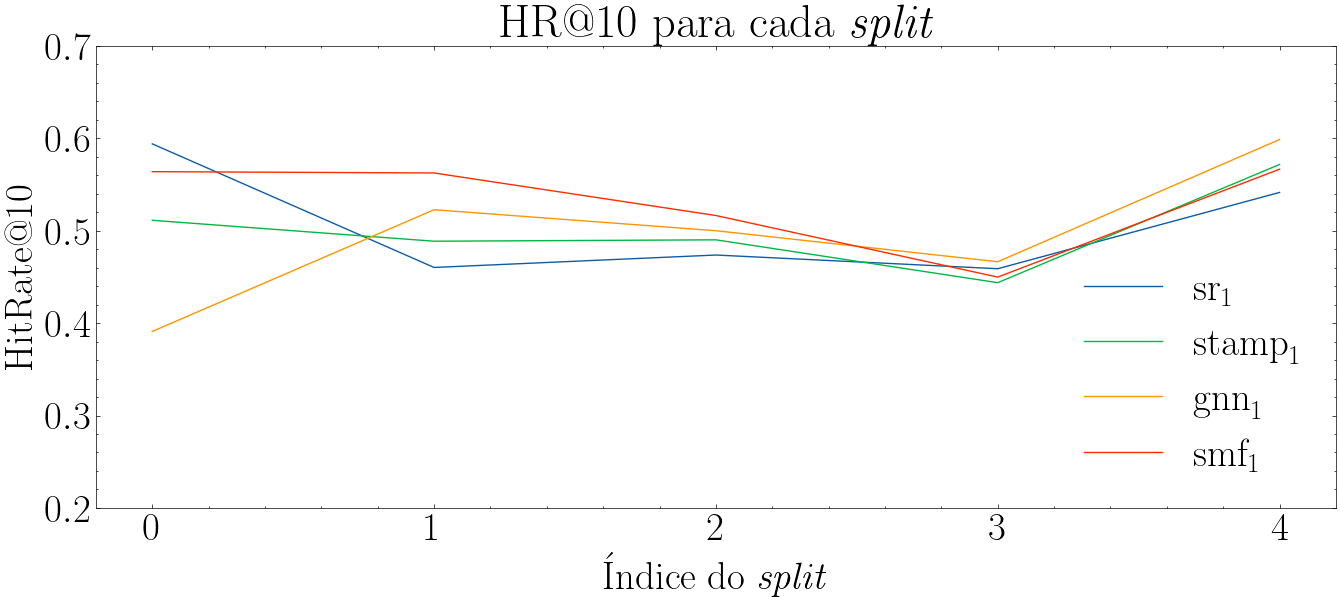
\includegraphics[width=1\textwidth]{chapters/chap04/images/hr10_splits.png}
  \caption{HR@10 em cada janela para alguns modelos da tabela
  \ref{tab:windowed_next_item_all}.}
  \label{fig:next-item-single}
\end{figure}


A figura \ref{fig:progressao} apresenta a progressão do HR e MRR conforme a
quantidade de valores preditos. É possível observar que as pontuações tendem
a convergir.
\newpage

\begin{figure}[htbp]
  \hfill
  \subfigure{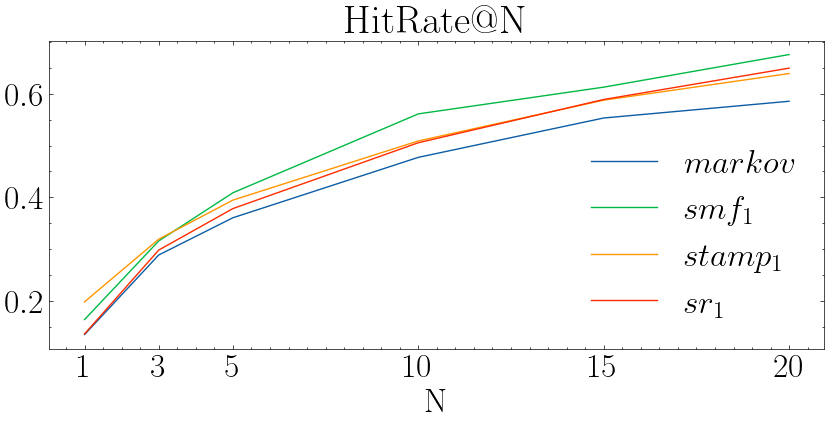
\includegraphics[width=7cm]{chapters/chap04/images/pplotHitRate_n.png}}
  \hfill
  \subfigure{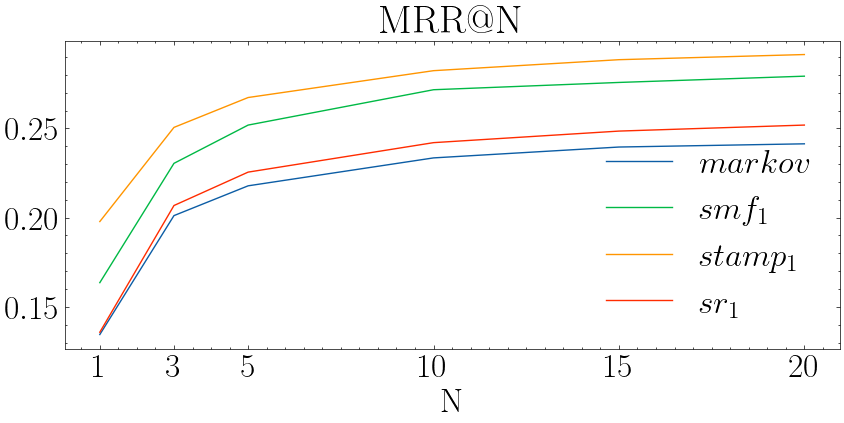
\includegraphics[width=7cm]{chapters/chap04/images/pplotMRR_n.png}}
  \hfill
  \caption{Progressão do HR e MRR conforme a quantidade de valores preditos.}
  \label{fig:progressao}
  \end{figure}

\subsection{Abordagem \textit{windowed}, \textit{session-based}, \textit{remaining-items}}
Para a abordgem \textit{remaining-items}, foi realizada uma nova otimização
considerando a métrica MAP@10. Essa nova otimização é necessária dado que a
avaliação do modelo é realizada com métricas que avaliam os acertos nos demais
itens subsequentes, e não para um único item.

Dessa forma, os modelos com nome subscrito aqui presentes possuem hiperparâmetros
distintos da abordagem anterior, constando no apêndice.

\begin{table}[htbp]
  \centering
  \begin{tabular}{|l|l|l|l|l|l|l|}
    \hline
    Modelos & P@10 & R@10 & NDCG@10 & MAP@10 & Cov@10 & Pop@10 \\
    \hline
    rpop & $\mathbf{0,086}$ & $\mathbf{0,361}$ & \textbf{0,240} & $\mathbf{0,042}$ & 0,065 & 0,355 \\
    \hline
    pop & 0,075 & 0,326 & 0,220 & 0,038 & 0,034 & 0,493 \\
    \hline
    spop & 0,065 & 0,298 & 0,179 & 0,032 & 0,235 & 0,456 \\
    \hline
    random & 0,007 & 0,033 & 0,018 & 0,003 & $\mathbf{1,000}$ & $\mathbf{0,046}$ \\
    \hline
  \end{tabular}
  \caption{Resultados para os modelos de popularidade.}
  \label{tab:model_metrics}
\end{table}


\begin{table}[htbp]
  \centering
  \begin{tabular}{|l|l|l|l|l|l|l|}
    \hline
    Model & P@10 & R@10 & NDCG@10 & MAP@10 & Cov@10 & Pop@10 \\
    \hline
%     "",Metrics,Precision@10:,Recall@10:,NDCG@10:,MAP@10:,Coverage@10:,Popularity@10:
% 0,ct,0.103479,0.479429,0.367222,0.056432,0.374663,0.395848
    ct & \textbf{0,103} & \textbf{0,479} & \textbf{0,367} & \textbf{0,056} & 0,375 & 0,396 \\
    \hline
    $\text{smf}_1$ & 0,100 & 0,450 & 0,333 & 0,055 & 0,242 & 0,347 \\
    \hline
    $\text{smf}_2$ & 0,100 & 0,459 & 0,338 & 0,055 & 0,343 &\textbf{ 0,321} \\
    \hline
    fpmc & 0,086 & 0,403 & 0,267 & 0,044 & 0,607 & 0,345 \\
    \hline
    bprmf & 0,084 & 0,389 & 0,260 & 0,044 & 0,612 & 0,347 \\
    \hline
    fism & 0,083 & 0,396 & 0,264 & 0,045 & \textbf{0,616} & 0,346 \\
    \hline
    fossil & 0,081 & 0,373 & 0,252 & 0,042 & 0,606 & 0,346 \\
    \hline
  \end{tabular}
  \caption{Resultados para modelos de fatoração de matrizes.}

\end{table}
\begin{table}[htbp]
  \centering
  \begin{tabular}{|l|l|l|l|l|l|l|l|}
    \hline
    Modelo & P@10 & R@10 & NDCG@10 & MAP@10 & Cov@10 & Pop@10 \\
    \hline
    $\text{vsknn}_1$ & $\mathbf{0,101}$ & 0,471 & 0,301 & 0,057 & 0,477 & 0,295 \\
    \hline
    $\text{stan}_1$ & 0,100 & $\mathbf{0,482}$ & $\mathbf{0,303}$ & $\mathbf{0,059}$ & 0,464 & 0,304 \\
    \hline
    $\text{stan}_2$ & 0,099 & 0,469 & 0,296 & 0,057 & 0,467 & 0,316 \\
    \hline
    $\text{vstan}_1$ & 0,098 & 0,463 & 0,296 & 0,057 & 0,468 & 0,319 \\
    \hline
    $\text{sknn}_1$ & 0,097 & 0,471 & 0,294 & 0,056 & 0,468 & 0,318 \\
    \hline
    $\text{sknn}_2$ & 0,095 & 0,487 & 0,300 & 0,057 & 0,540 & 0,260 \\
    \hline
    $\text{vsknn}_2$ & 0,091 & 0,426 & 0,268 & 0,051 & 0,542 & 0,216 \\
    \hline
    $\text{vstan}_2$ & 0,088 & 0,441 & 0,266 & 0,052 & \textbf{0,571} & \textbf{0,212} \\
    \hline
  \end{tabular}
  \caption{Resultados das métricas para os modelos baseados em vizinhança.}
  \label{tab_model_metrics}
\end{table}

\begin{table}[htbp]
  \centering
  \begin{tabular}{|c|c|c|c|c|c|c|}
    \hline
     Modelos & P@10 & R@10 & NDCG@10 & MAP@10 & Cov@10 & Pop@10 \\
    \hline
    $\text{sr}_1$ & \textbf{0,104} & 0,457 & 0,337 & \textbf{0,057} & 0,434 & 0,286 \\
    \hline
    ct & 0,103 & \textbf{0,479} & \textbf{0,367} & 0,056 & 0,375 & 0,396 \\
    \hline
    $\text{sr}_2$ & 0,101 & 0,455 & 0,332 & 0,056 & 0,453 & 0,273 \\
    \hline
     ar & 0,098 & 0,442 & 0,331 & 0,054 & \textbf{0,455} & 0,300 \\
    \hline
     markov & 0,091 & 0,420 & 0,310 & 0,050 & 0,438 & \textbf{0,257} \\
    \hline
  \end{tabular}
  \caption{Resultados para regras de associação.}
  \label{tab_model_results}
\end{table}




\begin{table}[htbp]
  \centering
  \begin{tabular}{|c|c|c|c|c|c|c|}
    \hline
    Modelo & P@10 & R@10 & NDCG@10 & MAP@10 & Cov@10 & Pop@10 \\
    \hline
    GNN & \textbf{0,097} & \textbf{0,455} & \textbf{0,359} & \textbf{0,056} & 0,603 & 0,272 \\
    \hline
    $\text{STAMP}_2$ & \textbf{0,097} & 0,453 & 0,341 & 0,052 & 0,608 & 0,285 \\
    \hline
    $\text{STAMP}_1$ & 0,096 & 0,445 & 0,331 & 0,052 & 0,560 & 0,286 \\
    \hline
    $\text{NextItNet}_2$ & 0,095 & 0,435 & 0,310 & 0,051 & 0,531 & 0,293 \\
    \hline
    $\text{NextItNet}_1$ & 0,090 & 0,427 & 0,314 & 0,048 & 0,321 & 0,340 \\
    \hline
    $\text{NARM}_2$ & 0,079 & 0,392 & 0,286 & 0,043 & 0,641 & 0,256 \\
    \hline
    $\text{NARM}_1$ & 0,079 & 0,381 & 0,266 & 0,042 & 0,610 & 0,256 \\
    \hline
    $\text{CSRM}_2$ & 0,067 & 0,310 & 0,209 & 0,034 & 0,459 & 0,278 \\
    \hline
    $\text{CSRM}_1$ & 0,064 & 0,314 & 0,210 & 0,033 & 0,473 & 0,279 \\
    \hline
    $\text{GRU4Rec}_2$ & 0,017 & 0,081 & 0,053 & 0,008 & 0,416 & 0,026 \\
    \hline
    $\text{GRU4Rec}_1$ & 0,008 & 0,035 & 0,022 & 0,003 & \textbf{0,707} & \textbf{0,022} \\
    \hline
  \end{tabular}
  \caption{Resultados para redes neurais.}
\end{table}

\newpage

\subsection{Abordagem \textit{windowed}, \textit{session-aware}, \textit{next-item}}

Em seguida, são apresentados os resultados obtidos com a abordagem
\textit{windowed} e \textit{session-aware}. Os modelos passaram por otimização
de seus hiperparâmetros, cujos resultados constam no apêndice.

A tabela \ref{tab:windowed_data_session_aware} apresenta os conjuntos de treino
e teste separados em cinco janelas. Novamente, é possível observar o aumento
gradual da quantidade de eventos, sessões e itens ao longo dos \textit{splits}.

Metade dos modelos \textit{session-aware} apresentam resultados que superam
todos os modelos da abordagem \textit{session-based}. O modelo de regras de
sequência \textit{session-aware} é o único modelo com MRR@5 acima de 0,3. Os
modelos NARM e iiRNN também obtiveram MRR@10 superior a 0,3. O modelo vsKNN
\textit{session-aware} obteve um incremento considerável no HR@10 quando
comparado ao seu equivalente \textit{session-based}.

\begin{table}[htbp]
  \begin{tabular}{|l|l|l|l|l|l|l|l|}
    \hline
    Modelo & HR@5 & HR@10 & MRR@5 & MRR@10 & Cov@10 & Pop@10 & $\Delta t_{treino} [s]$ \\
    \hline
    USR & $\mathbf{0,487}$ & 0,627 & $\mathbf{0,325}$ & $\mathbf{0,344}$ & 0,812 & 0,242 & 0,112 \\
    \hline
    USTAN & 0,484 & 0,626 & 0,256 & 0,275 & 0,724 & 0,298 & 108,7 \\
    \hline
    UVSKNN & 0,474 & $\mathbf{0,648}$ & 0,243 & 0,267 & 0,697 & 0,300 & 0,079 \\
    \hline
    UNARM & 0,465 & 0,610 & 0,296 & 0,315 & 0,832 & 0,236 & 244,6 \\
    \hline
    iiRNN & 0,442 & 0,554 & 0,293 & 0,308 & 0,721 & 0,230 & 145,7 \\
    \hline
    NSAR & 0,393 & 0,522 & 0,253 & 0,271 & 0,586 & 0,279 & 77,2 \\
    \hline
    NCFS & 0,368 & 0,493 & 0,225 & 0,241 & 0,452 & 0,370 & 21,6 \\
    \hline
    UGRU4Rec & 0,358 & 0,471 & 0,238 & 0,253 & $\mathbf{0,910}$ & 0,116 & 44,4 \\
    \hline
    SHAN & 0,343 & 0,471 & 0,202 & 0,219 & 0,470 & 0,309 & 642,3 \\
    \hline
    HGRU4Rec & 0,296 & 0,377 & 0,190 & 0,201 & 0,762 & $\mathbf{0,113}$ & 14,5 \\
    \hline
    \end{tabular}
  \caption{Resultado dos modelos \textit{session-aware} na abordagem
  \textit{windowed}, avaliando o próximo item da sessão. Valores exibidos são a
  média dos cinco \textit{splits}. Modelos ordenados por HR@5. }
\end{table}
\newpage

\begin{table}[htbp]
  \centering
  \begin{tabular}{|c|c|c|c|c|c|c|}
    \hline
    Conjunto & Índice & Eventos & Usuários & Sessões & Itens & Data -- 2023\\
    \hline
    Treino & 1 & 2705 & 76 & 721 & 124 & 01/08 a 13/03\\
    \hline
    Teste & 1 & 245 & 73 & 73 & 75 & 16/03 a 13/03\\
    \hline
    Validação -- Treino & 1 & 2427 & 76 & 645 & 119 & 01/08 a 12/03\\
    \hline
    Validação -- Teste & 1 & 269 & 74 & 74 & 75 & 16/01 a 13/03\\
    \hline
    Treino & 2 & 3463 & 74 & 898 & 160 & 14/03 a 17/05\\
    \hline
    Teste & 2 & 256 & 73 & 73 & 87 & 20/03 a 17/05\\
    \hline
    Validação -- Treino & 2 & 3186 & 74 & 824 & 158 & 14/03 a 17/05\\
    \hline
    Validação -- Teste & 2 & 275 & 74 & 74 & 93 & 20/03 a 17/05\\    
    \hline
    Treino & 3 & 6620 & 109 & 1520 & 270 & 18/05 a 21/06\\
    \hline
    Teste & 3 & 368 & 108 & 108 & 123 & 01/06 a 21/07\\
    \hline
    Validação -- Treino & 3 & 6226 & 109 & 1411 & 265 & 18/05 a 21/07\\
    \hline
    Validação -- Teste & 3 & 386 & 106 & 106 & 130 & 23/05 a 21/07\\
    \hline
    Treino & 4 & 15180 & 308 & 3143 & 581 & 21/07 a 24/09\\
    \hline
    Teste & 4 & 1614 & 305 & 305 & 318 & 23/07 a 24/09\\
    \hline
    Validação -- Treino & 4 & 13483 & 308 & 2835 & 556 & 21/07 a 24/09\\
    \hline
    Validação -- Teste & 4 & 1630 & 298 & 298 & 305 & 22/07 a 24/09\\
    \hline
    Treinamento & 5 & 23244 & 646 & 4369 & 1092 & 24/09 a 28/11\\
    \hline
    Teste & 5 & 3317 & 629 & 629 & 670 & 30/09 a 28/11\\
    \hline
    Validação -- Treino & 5 & 19820 & 646 & 3723 & 1027 & 24/09 a 28/11\\
    \hline
    Validação -- Teste & 5 & 3288 & 625 & 625 & 676 & 26/09 a 28/11\\
    \hline
  \end{tabular}
  \caption{Conjuntos de treino, teste e validação separados em cinco janelas para abordagem \textit{session-aware}.}
  \label{tab:windowed_data_session_aware}
\end{table}

% \section{Tratamento dos dados}
% Sob a perspectiva comercial, o seguinte indício sustenta que um SBRS pode
% aumentar a taxa de sessões publicadas pelos usuários do Indaband: apenas 1.146
% (7,77\%) das 14.750 sessões criadas em 2023 até 13 de agosto contém no mínimo um
% convite emitido. Afunilando ainda mais, a análise das taxas de publicação indica
% que as sessões com ao menos um convite aceito, que são apenas 349 (2,37\%) das
% 14.750 sessões totais criadas, tem maior taxa de publicação se comparada ao
% conjunto de todas as sessões. Portanto, uma forma simples de aumentar a taxa de
% publicação geral da plataforma é permitir que o conjunto de sessões com
% convidados seja maior, o que pode ser incentivado ao integrar um SBRS ao
% aplicativo.

% Sob a perspectiva de viabilidade técnica, de todas as 14.750 sessões criadas
% em 2023 até 13 de agosto, 6.857 (46,5\%) foram criadas com ao menos dois
% usuários que gravaram as faixas existentes. Isso é possível a partir da
% funcionalidade de \textit{fork}, que permite a cópia de uma sessão publicada
% com suas faixas originais. Basta um novo usuário versionar uma sessão com uma
% única faixa de outro usuário para que exista associações entre esse novo
% usuário e os demais que o segundo usuário já tenha colaborado.

% \vspace{0.2cm}
% \begin{figure}[H]
%       \centering
%       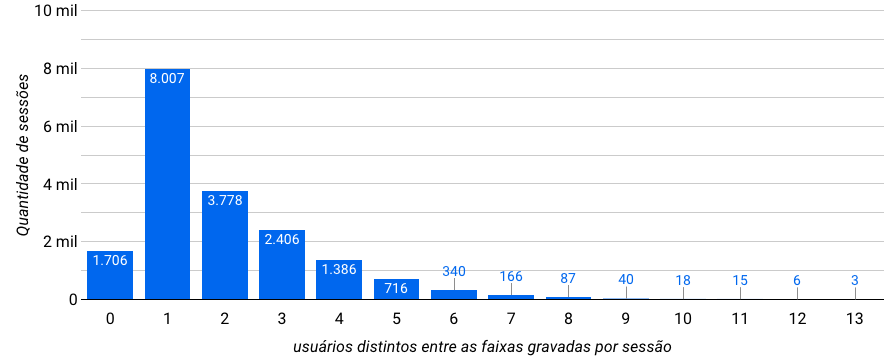
\includegraphics[width=1\textwidth]{chapters/chap01/images/plots/users.png}\vfill
%       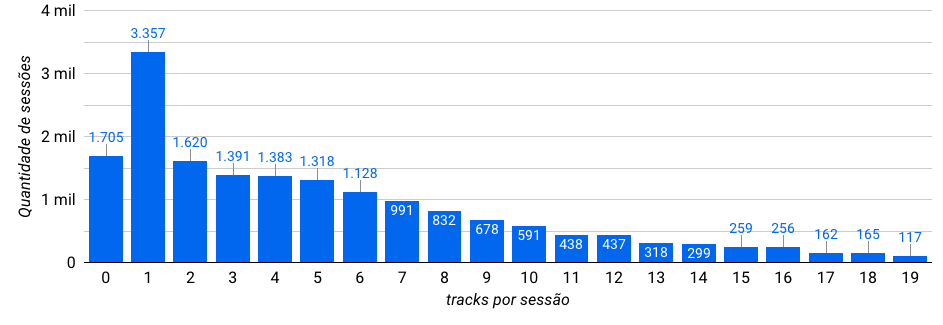
\includegraphics[width=1\textwidth]{chapters/chap01/images/plots/tracks.png}
%       \caption{Dados de sessões em 2023 até o presente momento. A quantidade de \textit{tracks}
%        e usuários por sessão sustenta a viabilidade técnica de um modelo de
%        aprendizado de máquina para a recomendação de convites.}
%       \label{fig:combined}
%   \end{figure}
% \vspace{0.2cm}

% \vspace{0.2cm}
% \begin{figure}[ht]
%     \centering
%     \begin{tikzpicture}
%     \pie[ sum=auto, radius=1.4, color={blue!70, orange!70}, after number=\%,
%       explode={0, 0.1}, text={}, pos={0,-1}, ]{ 41.3/Publicadas, 58.7/Não
%       Publicadas } \node[align=center] at (0,-3) {Total de Sessões: 14.750};
%     \end{tikzpicture}
%     \hspace{1cm} 
%     \begin{tikzpicture}
%     \pie[ sum=auto, radius=0.8, color={blue!70, orange!70}, after number=\%,
%       explode={0, 0.1}, text=legend, pos={0,-1}, ]{ 48.4/Publicadas, 51.6/Não
%       Publicadas } \node[align=center] at (0,-3) {Sessões com 1 convite aceito
%       ou mais: 349};
%     \end{tikzpicture}
%     \caption{Sessões e convites enviados. 01/01/2023 a 13/08/2023. Sessões com convites aceitos têm maior taxa de publicação se comparadas ao conjunto completo.}
%     \end{figure}
%     \vspace{0.2cm}
 
